\chapter{Method}

Prior to designing the game, background information was collected on the developer team's, as well as other people's, views and expectations on a new Tower Defense game. A number of existing well-known tower defense games were also tested and discussed to get a general idea of which features that are desirable. The design process included discussions of different ideas, drawing of mind maps and draft UML-diagrams.

The development was done in Eclipse IDE with the Android SDK-plugin. The program language Java was used. Included in Android SDK is an emulator which made it possible to test code directly on the computer.

The implementation was done using an agile development approach, in the sense that we worked in small iterations and changed the requirements continuously during the development process. To make the project easier to maintain, the distributed subversion management system Git was used.

Code convention was used to make the code easier to understand within the development group or for otherdevelopers that might work on the system later on. 

%----------------------------------------------------------
\section{Interviews}

Interviews were used as a tool in two different stages of the development; the research stage and the final testing stage.

Interviews were conducted to get a better picture of what makes a Tower Defense game good. The interviewees where people that play games regularly and had prior experience of playing Tower Defense games. Ten interviews were conducted, following an unstructured interview template with mainly open questions. The full interview template is found in Appendix C.1. 

The interviews provided some insight into peoples thoughts and the statements from the participants were used to make important design decisions. The interviews made it obvious that obvious that everyone had their own opinion on which features a good game should include, but several statements were general and helped avoiding common mistakes. 

In the final stage of development, ten more interviews were conducted to evaluate the resulting game. The template can be found in Appendix C.2. The answers helped finding areas that needed improvement.
%----------------------------------------------------------
\section{Android development environment}

Developing Android applications requires Java Development Kit (JDK) and an Integrated Development Environment (IDE). Google recommends Eclipse with Android Development Tools (ADT). The ADT is a plugin for Eclipse that allows easy creation and management of Android projects. \citep{Android}

The Eclipse Foundation is an open-source community originally created by IBM in 2001. Its most popular IDE Package is the Eclipse IDE for Java Enterprise Edition (EE) Developers that currently have over 1.2 million downloads. Eclipse IDE is free to use and allows the users to easily create Java applications. \citep{Eclipse}

Figure ~\ref{fig:eclipseIDE} shows a screenshot of a project in Eclipse. The left panel displays the project files and the center panel displays the currently open file. At the bottom there is a console showing the status of the different tasks that Eclipse is performing: log messages, error messages etcetera. To the right is an outline of the methods and variables in the current file. This helps the user to easily overview and navigate the code.

%-------
%- Image eclipse
%-------
\begin{figure}[here]
\begin{center}
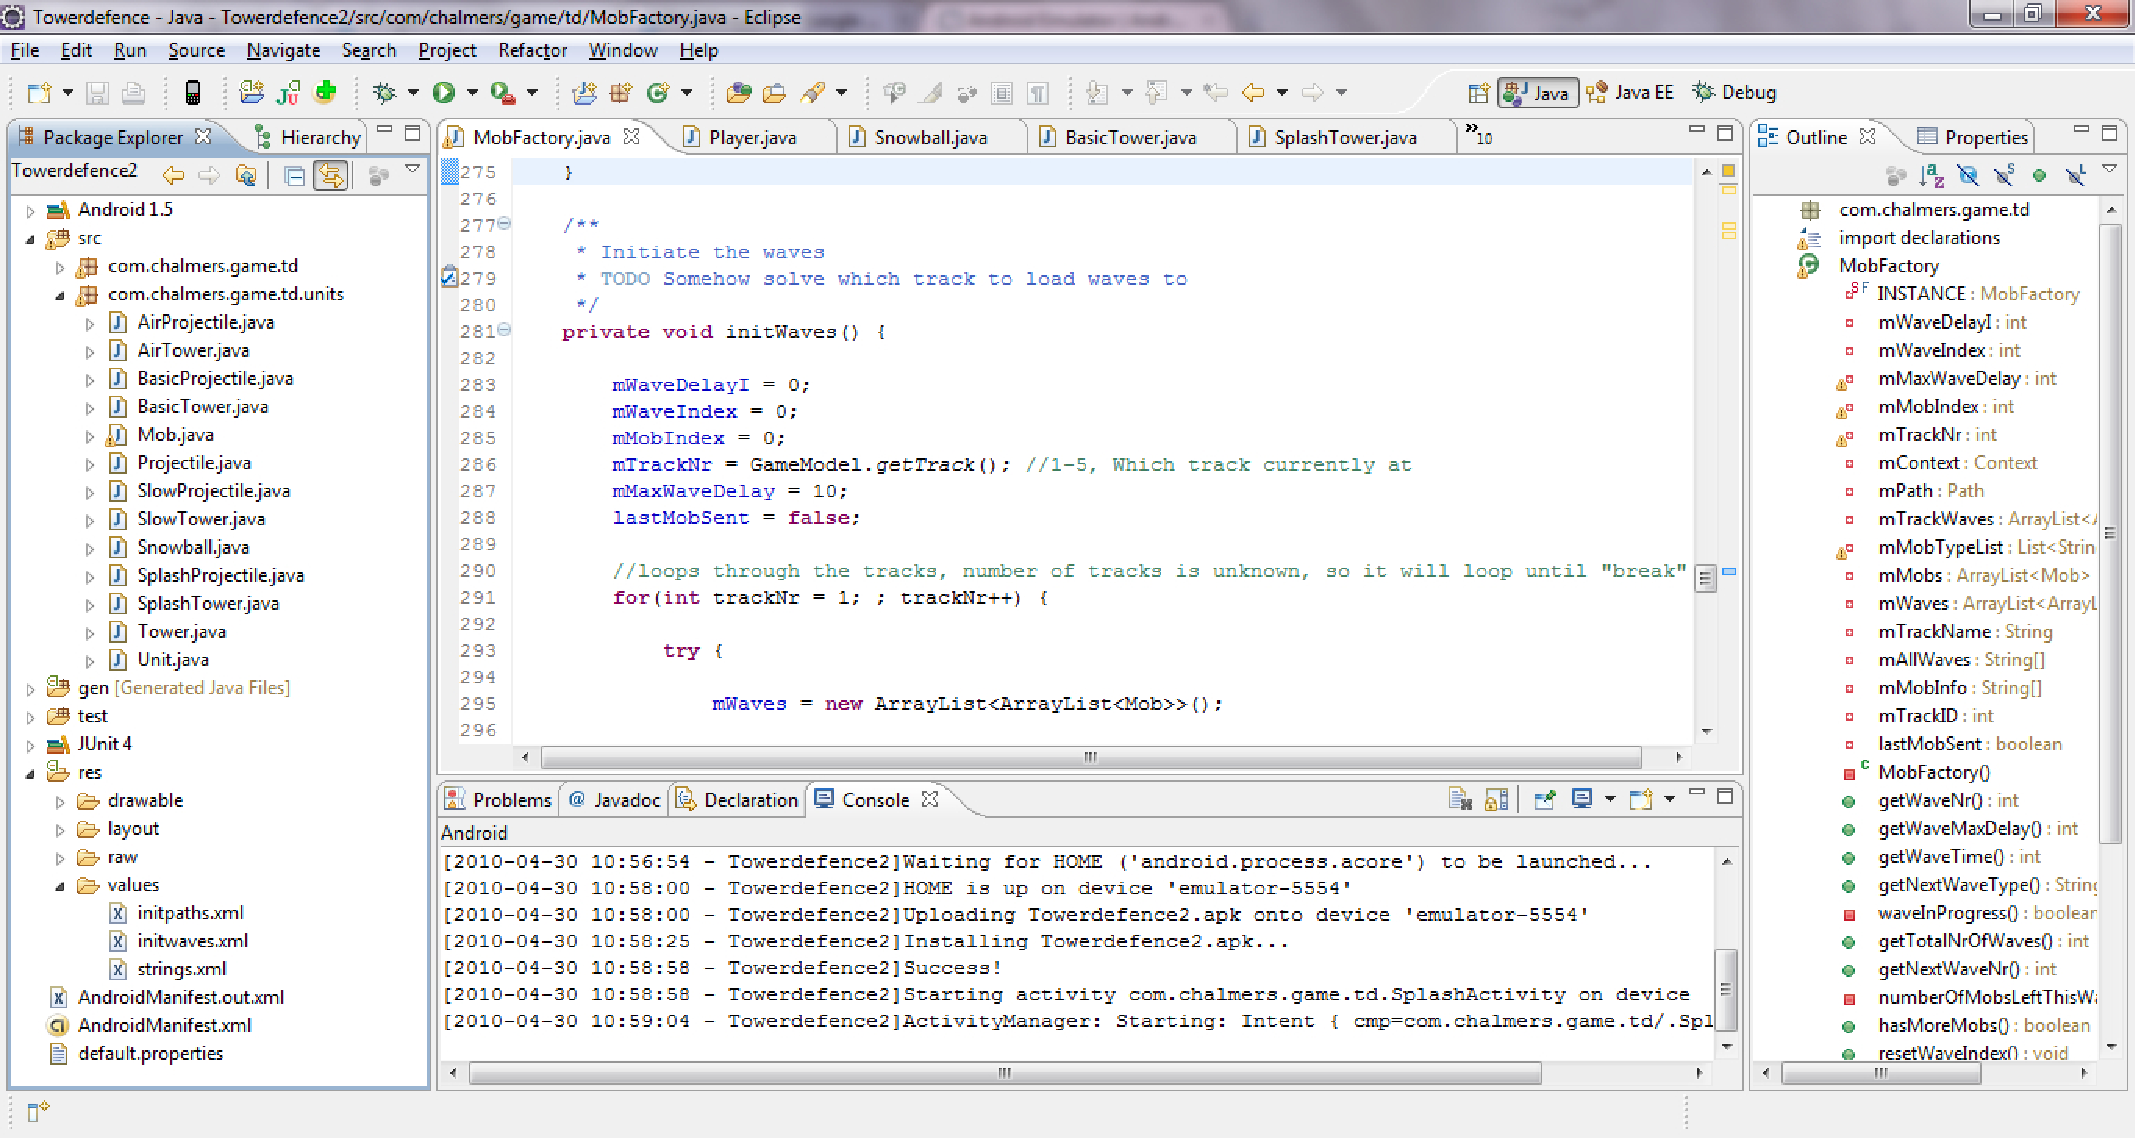
\includegraphics[scale=0.3]{pics/chapters/chapter2/eclipse}
\end{center}
\caption{Eclipse Intergrated Development Environment}
\label{fig:eclipseIDE}
\end{figure}
%-------

The Android Development Kit includes an Android emulator (figure ~\ref{fig:androidEmulator}). This allows the developer to test her applications without the use of an actual phone. It supports a majority of the functionalities of a real phone, such as simulating SMS, phone calls, events and geographic locations (like GPS navigation). The mouse can be used to click on the screen to emulate usage of the touchscreen of the device, and virtual buttons represent the normally available hardware buttons on a physical phone (figure ~\ref{fig:androidEmulator}) . The emulator can be set up to use different resolutions and different versions of Android, allowing the developer to verify software compatibility. \citep{Android}

%-------
%- Image Android emulator
%-------
\begin{figure}[here]
\begin{center}
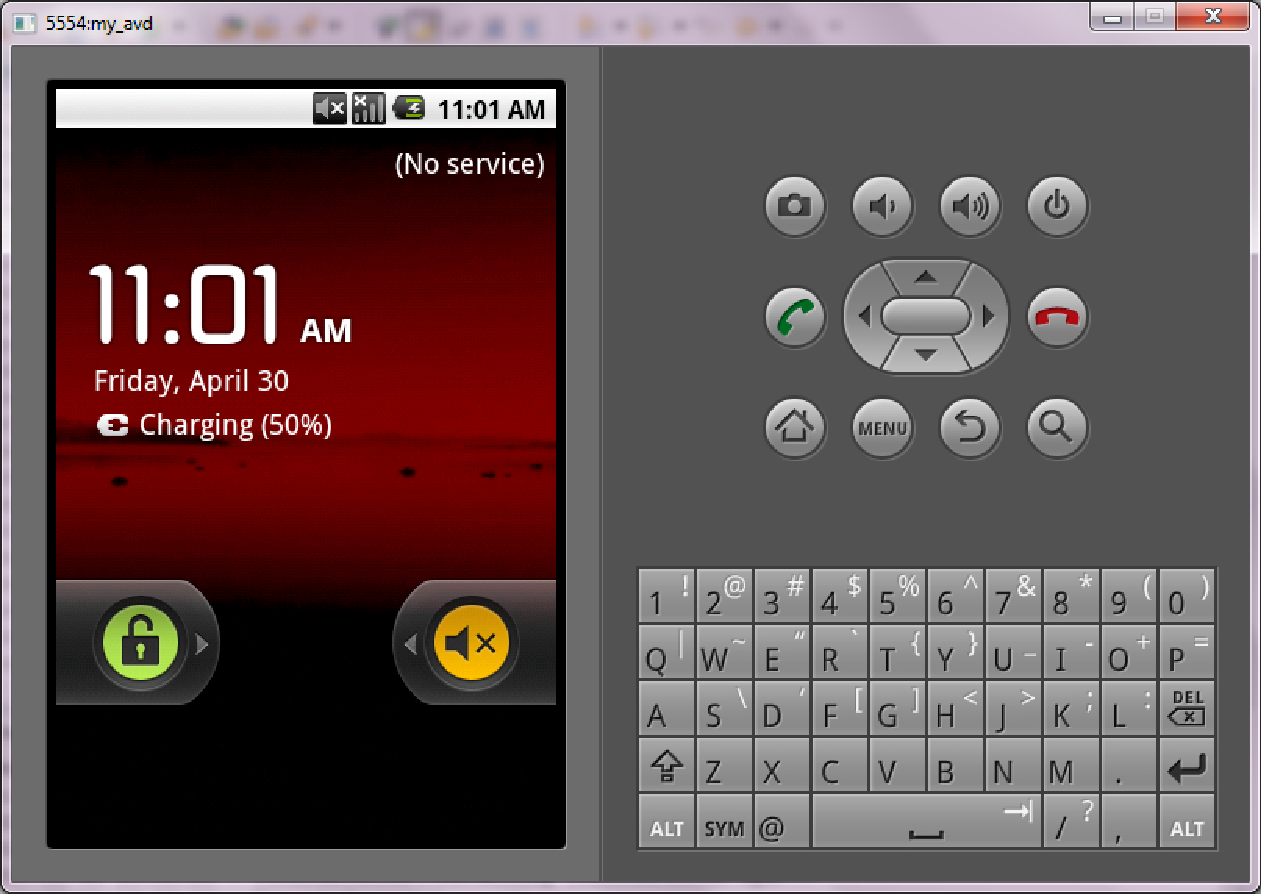
\includegraphics[scale=0.4]{pics/chapters/chapter2/emulator}
\end{center}
\caption{The Android emulator}
\label{fig:androidEmulator}
\end{figure}
%-------

%----------------------------------------------------------
\section{Code convention}

Code convention is a huge subject of its own, and can be divided into subcategories such as style, language and programming practices. When developing large software systems it is important to follow a common code style convention. A main reason for this is to make the code easier to understand for developers that might work on the system later on. This involves choosing suitable names for variables and classes, as well as making similar choices of code constructions. 

Android is an open source project, and a set of rules have been created to keep a common style between developers. These rules are intended for contributors to the android platform itself. Even though they are not a requirement for application development, they are still well thought out and adapted to the Android environment. For this reason these rules were used as guidelines for this project as well. Some of these could be seen as common sense while others add extra readability beyond what is common in Java programming.

The following paragraphs describe some of the important style conventions that were used, and how they differ from the android contributor rules

\subsubsection{Javadoc and comments}

Javadoc comments were continuously added to the code, using Java's standard format as suggested by Android. Non-javadoc comments were used as well to clearify the code and increase maintainability.

\subsubsection{Short methods}

Long methods were broken down into shorter ones to increase readability where possible. One good example of this is the method onDraw() (figure ~\ref{fig:codeExOnDraw}) in the class GameView. This calls several submethods that draws different parts of the game, instead of drawing everything inside one single method.

%--------------------------------
%- Code snippet onDraw
%--------------------------------
\begin{figure}[htb]
\begin{small}
\verbatiminput{code/onDraw.java}
\end{small}
\caption{Pseudocode for the method onDraw()}
\label{fig:codeExOnDraw}
\end{figure}
%--------------------------------

\subsubsection{Fields}

Fields should either be at the top of the file or immediately before the methods that use them, according to the Android development rules. All fields in this project were declared at the top of the file. Java code conventions recommend field declaration in the following order: "First the public class variables, then the protected, then package level (no access modifier), and then the private." \citep{Sun}.

\subsubsection{Limit the scope of local variables}

Local variables were initialized on the same line as they are declared if possible, and also as close as possible to where they are actually used, as suggested by Android.

\subsubsection{Indentation}

The rules recommend using four spaces instead of tabulations. However, since this project was made entirely in Eclipse, normal tabs were used instead. This is the default way that Eclipce handles indentation and it is facilitated by using auto-indenting options.

\subsubsection{Field names and other names}

In the project the following field name rules were followed strictly:

%---------------
\begin{itemize}

\item Non-public, non-static field names start with m.
\item Static field names start with s.
\item Other fields start with a lower case letter.
\item Public static final fields (constants) are ALL\_CAPS\_WITH\_UNDERSCORES.

\end{itemize}
%---------------

Additionally, the field names were carefully chosen so that their purpose was clear, and use of ambiguous names or shortenings was avoided.

\subsubsection{TODO annotation}

The TODO annotation was used during the coding process, to mark unfinished sections in the code. Eclipse automatically recognizes the TODO-comments, making it easier for the developer to find them by marking their locations on the scrollbar while browsing the code.

\subsubsection{Logging}

Logging was used for debugging purposes. The log method made it possible to spot non-functional sections in the code. Debug messages were marked as verbose, to ensure that they were only compiled in debug mode. In that way they would not affect the performance of the game.
%----------------------------------------------------------
\section{Git - A version control system}

When developing software in teams, a system to manage and synchronize the source code is needed. It ensures that everyone in the project is working on the latest version of the system. Git was used in this project to fulfill this purpose.

When working with Git each developer has one local repository on their computer. Changes made to the code are then copied between the other developers local repositories. This does not force the users to have a dedicated server to store a central repository. Instead Git users are free to store their repositories anywhere. \citep{Git} 

Since Git allows the project to be stored locally on every developer's computer, work can be done on the implementation despite lack of internet access. Any system failure will affect only one individual, providing the project with an increased tolerance to any system breakdowns.
%----------------------------------------------------------